%%%%%%%%%%%%%%%%%%%%%%%%%%%%%%%%%%%%%%%%%%%%%%%%%%%%%%%%%%%%%%%%%%%%%%%%%%%%%%
\chapter{Présentation et Contexte général}
%%%%%%%%%%%%%%%%%%%%%%%%%%%%%%%%%%%%%%%%%%%%%%%%%%%%%%%%%%%%%%%%%%%%%%%%%%%%%%

\section{Introduction}

Ce chapitre présente le contexte institutionnel et technologique dans lequel s'inscrit le présent projet. Il débute par une présentation du Groupement Sanitaire Territorial Tanger--Tétouan--Al Hoceïma (GST-TTA), organisme d'accueil ayant encadré la réalisation du projet. Il expose ensuite les principales missions de cette institution, son organisation ainsi que le rôle de la Direction de la Formation, de la Recherche et de l'Innovation, au sein de laquelle le projet a été développé.

Ce chapitre introduit également les enjeux liés à la transformation numérique du secteur de la santé et met en évidence les motivations ayant conduit au développement d'une plateforme intelligente d'analyse conversationnelle de données. L'analyse de l'existant permet d'identifier les limites des solutions actuelles, justifiant la formulation de la problématique et des objectifs du projet.

Enfin, ce chapitre présente l'organisation du travail à travers la structure de l'équipe projet, la répartition des tâches et la planification temporelle via un diagramme de Gantt.

\vspace{0.3cm}

%%%%%%%%%%%%%%%%%%%%%%%%%%%%%%%%%%%%%%%%%%%%%%%%%%%%%%%%%%%%%%%%%%%%%%%%%%%%%%
\section{Présentation de l'organisme d'accueil}
%%%%%%%%%%%%%%%%%%%%%%%%%%%%%%%%%%%%%%%%%%%%%%%%%%%%%%%%%%%%%%%%%%%%%%%%%%%%%%

\subsection{Présentation du GST-TTA}

Le présent projet de fin d'année a été réalisé au sein du \textbf{Groupement Sanitaire Territorial Tanger--Tétouan--Al Hoceïma (GST-TTA)}, établissement public de santé placé sous la tutelle du \textbf{Ministère de la Santé et de la Protection Sociale}.

Créé dans le cadre de la réforme du système national de santé et de la mise en œuvre de la régionalisation avancée, le GST-TTA constitue une nouvelle structure de gouvernance visant à améliorer la coordination des établissements de santé, renforcer la qualité des soins et optimiser la gestion des ressources hospitalières à l'échelle régionale.

Le Groupement couvre l'ensemble de la région Tanger--Tétouan--Al Hoceïma, représentant près de 3,7 millions d'habitants, et fédère plusieurs établissements hospitaliers, centres spécialisés ainsi que des structures de formation et de recherche.

Au-delà de ses missions de coordination, le GST-TTA conduit une politique de modernisation des systèmes d'information afin d'accompagner la transformation numérique des établissements de santé et de favoriser une prise de décision fondée sur l'exploitation des données.

\begin{figure}[H]
\centering
\begin{subfigure}{0.45\textwidth}
    \centering
    
\includegraphics[width=\textwidth]{images/logo-site-gst.png}
    \caption{Logo du GST-TTA}
    \label{fig:logo_gst}
\end{subfigure}
\hfill
\begin{subfigure}{0.45\textwidth}
    \centering
    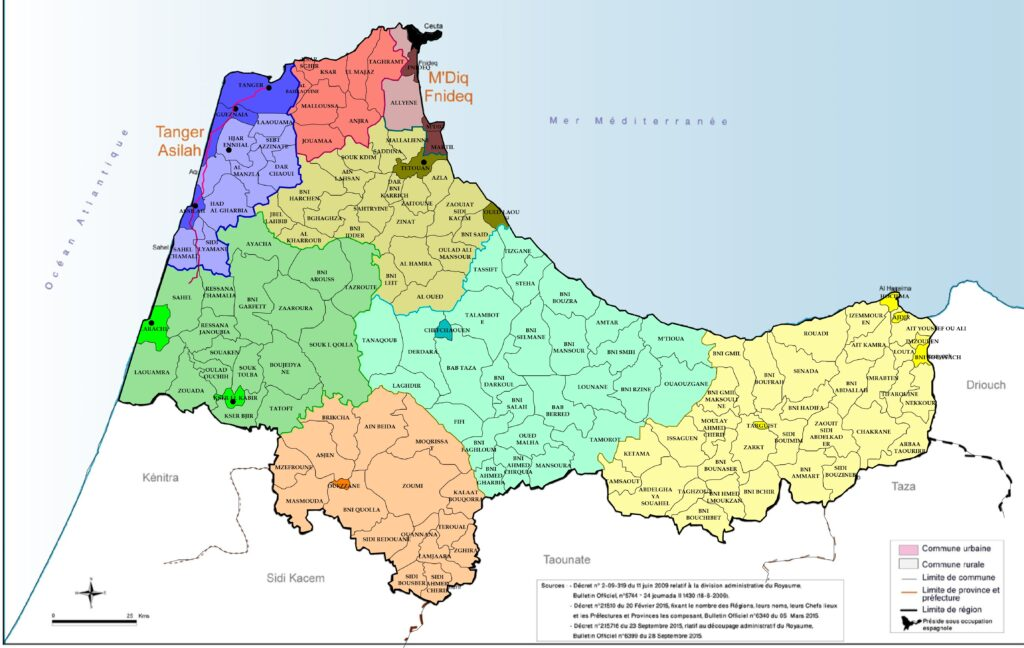
\includegraphics[width=\textwidth]{images/tanger-tetouan-al-houceima-region-map.jpeg}
    \caption{Carte de la région Tanger--Tétouan--Al Hoceïma}
    \label{fig:map-region}
\end{subfigure}
\caption{Présentation du Groupement Sanitaire Territorial Tanger--Tétouan--Al Hoceïma}
\label{fig:gst_presentation}
\end{figure}

%%%%%%%%%%%%%%%%%%%%%%%%%%%%%%%%%%%%%%%%%%%%%%%%%%%%%%%%%%%%%%%%%%%%%%%%%%%%%%
\subsection{Fiche signalétique}

Les principales informations relatives à l'organisme d'accueil sont présentées dans le tableau~\ref{tab:gst}.

\begin{table}[H]
\centering
\rowcolors{2}{LightGray}{white}
\begin{tabularx}{\textwidth}{>{\bfseries}p{4cm}X}
\toprule
\rowcolor{TableHeader}
\color{white}Élément & \color{white}Description \\
\midrule
Raison sociale & Groupement Sanitaire Territorial Tanger--Tétouan--Al Hoceïma (GST-TTA) \\
Tutelle & Ministère de la Santé et de la Protection Sociale \\
Statut juridique & Établissement public de santé, sous la tutelle de l'État \\
Région couverte & Tanger--Tétouan--Al Hoceïma \\
Population desservie & Environ 3,7 millions d'habitants \\
Siège & Tanger \\
Site web & \url{https://gst-tta.ma} \\
Direction d'accueil & Direction de la Formation, de la Recherche et de l'Innovation \\
\bottomrule
\end{tabularx}
\caption{Fiche signalétique du GST-TTA}
\label{tab:gst}
\end{table}

%%%%%%%%%%%%%%%%%%%%%%%%%%%%%%%%%%%%%%%%%%%%%%%%%%%%%%%%%%%%%%%%%%%%%%%%%%%%%%
\subsection{Missions}

Le GST-TTA assure la gouvernance des établissements de santé de la région et veille à l'amélioration continue de la qualité des services proposés aux citoyens.

Ses principales missions sont les suivantes :

\begin{itemize}
  \item coordonner les établissements hospitaliers de la région ;
  \item améliorer la qualité, la sécurité et la continuité des soins ;
  \item optimiser la gestion des ressources humaines, matérielles et financières ;
  \item accompagner la transformation numérique du système hospitalier ;
  \item promouvoir la recherche scientifique et l'innovation médicale ;
  \item développer les programmes de formation destinés aux professionnels de santé.
\end{itemize}

L'ensemble de ces missions contribue à renforcer l'efficacité du système de santé régional tout en favorisant l'introduction de solutions numériques innovantes. Ces missions, notamment l'accompagnement de la transformation numérique et la promotion de l'innovation, justifient le développement d'une plateforme comme celle présentée dans ce mémoire.

%%%%%%%%%%%%%%%%%%%%%%%%%%%%%%%%%%%%%%%%%%%%%%%%%%%%%%%%%%%%%%%%%%%%%%%%%%%%%%
\subsection{Organisation}

Le Groupement Sanitaire Territorial est organisé autour d'une direction générale appuyée par plusieurs directions fonctionnelles couvrant les domaines médicaux, administratifs, financiers, techniques ainsi que les activités liées à la recherche et à l'innovation.

Cette organisation favorise une gouvernance intégrée des établissements de santé et facilite la conduite de projets transversaux, notamment ceux liés à la transformation numérique.

\begin{figure}[H]
\centering
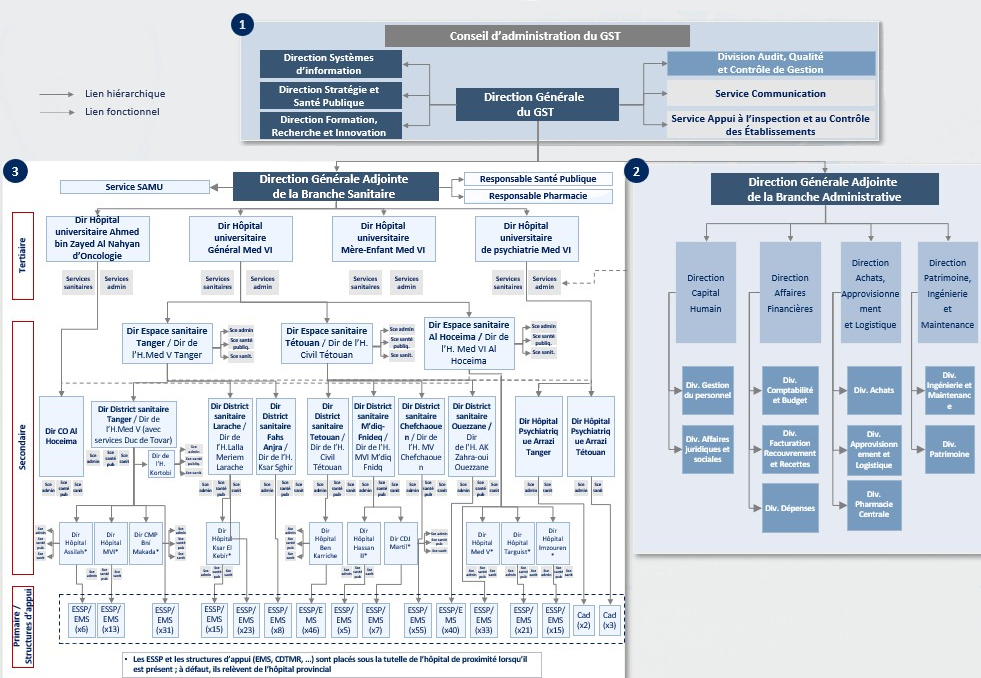
\includegraphics[width=0.92\textwidth]{images/3-Organigramme-general-GST-TTA.jpg}
\caption{Organigramme du Groupement Sanitaire Territorial Tanger--Tétouan--Al Hoceïma}
\label{fig:organigramme_gst}
\end{figure}

%%%%%%%%%%%%%%%%%%%%%%%%%%%%%%%%%%%%%%%%%%%%%%%%%%%%%%%%%%%%%%%%%%%%%%%%%%%%%%
\subsection{Direction de la Formation, de la Recherche et de l'Innovation}

Le projet a été réalisé au sein de la \textbf{Direction de la Formation, de la Recherche et de l'Innovation (DFRI)}.

Cette direction constitue un acteur majeur de la stratégie d'innovation du Groupement. Elle accompagne les établissements de santé dans leurs activités de formation, coordonne les projets de recherche et favorise le développement de solutions numériques répondant aux besoins du secteur hospitalier.

Parmi ses principales missions figurent :

\begin{itemize}
  \item la coordination des activités de formation ;
  \item le développement de projets de recherche scientifique ;
  \item la promotion de l'innovation technologique ;
  \item la valorisation des données de santé ;
  \item l'accompagnement des projets de transformation numérique.
\end{itemize}

Le développement de la plateforme présentée dans ce mémoire s'inscrit pleinement dans cette démarche de modernisation des outils d'aide à la décision fondés sur l'intelligence artificielle.

\begin{infobox}{Positionnement du projet}
Le projet a été réalisé au sein de la Direction de la Formation, de la Recherche et de l'Innovation du GST-TTA. Il contribue à la stratégie de transformation numérique de l'établissement en proposant une plateforme conversationnelle capable de faciliter l'exploitation des données grâce à l'intelligence artificielle générative.
\end{infobox}

%%%%%%%%%%%%%%%%%%%%%%%%%%%%%%%%%%%%%%%%%%%%%%%%%%%%%%%%%%%%%%%%%%%%%%%%%%%%%%
\section{Contexte général et analyse de l'existant}
%%%%%%%%%%%%%%%%%%%%%%%%%%%%%%%%%%%%%%%%%%%%%%%%%%%%%%%%%%%%%%%%%%%%%%%%%%%%%%

Le secteur de la santé connaît actuellement une profonde transformation numérique, marquée par la généralisation des systèmes d'information hospitaliers et la multiplication des données produites au quotidien. Cette évolution offre de nouvelles perspectives pour le pilotage des établissements de santé, l'amélioration de la qualité des soins et l'aide à la prise de décision.

Dans ce contexte, le Groupement Sanitaire Territorial Tanger--Tétouan--Al Hoceïma (GST-TTA) poursuit la modernisation de son infrastructure numérique afin de renforcer la gestion des établissements hospitaliers de la région. Toutefois, malgré la disponibilité d'un volume considérable de données, leur exploitation demeure complexe en raison des outils utilisés, de la diversité des sources d'information et des contraintes propres au domaine de la santé.

Cette section présente le contexte numérique du GST-TTA, les caractéristiques des données manipulées, le processus actuel d'analyse ainsi que les principales limites des solutions existantes.

%%%%%%%%%%%%%%%%%%%%%%%%%%%%%%%%%%%%%%%%%%%%%%%%%%%%%%%%%%%%%%%%%%%%%%%%%%%%%%
\subsection{Transformation numérique au GST-TTA}
%%%%%%%%%%%%%%%%%%%%%%%%%%%%%%%%%%%%%%%%%%%%%%%%%%%%%%%%%%%%%%%%%%%%%%%%%%%%%%

Dans le cadre de la réforme du système national de santé, le GST-TTA s'inscrit dans une stratégie visant à accélérer la transformation numérique des établissements hospitaliers de la région. Cette stratégie repose sur la modernisation des processus administratifs, le développement des systèmes d'information hospitaliers ainsi que l'amélioration de la gouvernance fondée sur les données.

La digitalisation progressive des activités permet aujourd'hui de dématérialiser de nombreux processus auparavant réalisés de manière manuelle, tout en facilitant la circulation de l'information entre les différents établissements du groupement.

Parmi les principaux axes de cette transformation figurent notamment :

\begin{itemize}
  \item la numérisation des processus administratifs et médicaux ;
  \item l'amélioration de la qualité et de la disponibilité des données ;
  \item le développement d'outils décisionnels ;
  \item la promotion des projets d'innovation numérique ;
  \item l'intégration progressive des technologies d'intelligence artificielle.
\end{itemize}

Cette évolution permet au GST-TTA de disposer d'un environnement numérique de plus en plus riche, capable de soutenir efficacement les activités de pilotage et d'aide à la décision.

%%%%%%%%%%%%%%%%%%%%%%%%%%%%%%%%%%%%%%%%%%%%%%%%%%%%%%%%%%%%%%%%%%%%%%%%%%%%%%
\subsection{Données et systèmes d'information hospitaliers}
%%%%%%%%%%%%%%%%%%%%%%%%%%%%%%%%%%%%%%%%%%%%%%%%%%%%%%%%%%%%%%%%%%%%%%%%%%%%%%

Les établissements hospitaliers produisent quotidiennement un volume important de données provenant de multiples systèmes d'information. Ces données concernent aussi bien les activités médicales que les aspects administratifs, logistiques et financiers.

Parmi les principales catégories de données exploitées, on distingue :

\begin{itemize}
  \item les données relatives aux patients et aux hospitalisations ;
  \item les consultations et actes médicaux ;
  \item les résultats des laboratoires ;
  \item les données de pharmacie ;
  \item les ressources humaines ;
  \item les indicateurs de performance hospitalière ;
  \item les données financières et logistiques.
\end{itemize}

Ces informations présentent plusieurs caractéristiques qui rendent leur exploitation particulièrement complexe :

\begin{itemize}
  \item un volume très important de données ;
  \item une mise à jour continue des informations ;
  \item une diversité des formats et des sources ;
  \item un niveau élevé de sensibilité nécessitant des mesures strictes de confidentialité ;
  \item des besoins croissants en matière d'analyse et de visualisation.
\end{itemize}

L'ensemble de ces données constitue une ressource stratégique permettant d'améliorer le suivi des activités hospitalières et de soutenir les décisions des responsables médicaux et administratifs.

%%%%%%%%%%%%%%%%%%%%%%%%%%%%%%%%%%%%%%%%%%%%%%%%%%%%%%%%%%%%%%%%%%%%%%%%%%%%%%
\subsection{Processus actuel et difficultés rencontrées}
%%%%%%%%%%%%%%%%%%%%%%%%%%%%%%%%%%%%%%%%%%%%%%%%%%%%%%%%%%%%%%%%%%%%%%%%%%%%%%

À l'heure actuelle, l'exploitation des données repose principalement sur une succession d'étapes réalisées à l'aide de plusieurs outils distincts.

Le processus classique comprend généralement :

\begin{enumerate}
  \item l'extraction des données depuis les différents systèmes d'information ;
  \item le nettoyage et la préparation des jeux de données ;
  \item la réalisation des traitements statistiques ;
  \item la création des tableaux et graphiques ;
  \item l'interprétation des résultats ;
  \item la rédaction des rapports.
\end{enumerate}

Bien que cette approche permette d'obtenir les analyses souhaitées, elle présente plusieurs inconvénients majeurs.

Les utilisateurs doivent souvent maîtriser plusieurs logiciels spécialisés tels que Microsoft Excel, SQL, Python ou encore Power BI. Cette multiplicité d'outils implique des manipulations répétitives, augmente les risques d'erreurs et allonge considérablement le temps nécessaire à la production des résultats.

Par ailleurs, la majorité des professionnels de santé ne disposent pas nécessairement des compétences techniques requises pour réaliser des analyses complexes, ce qui limite leur autonomie dans l'exploitation des données et crée une dépendance vis-à-vis des services spécialisés.

%%%%%%%%%%%%%%%%%%%%%%%%%%%%%%%%%%%%%%%%%%%%%%%%%%%%%%%%%%%%%%%%%%%%%%%%%%%%%%
\subsection{Limites des solutions existantes}
%%%%%%%%%%%%%%%%%%%%%%%%%%%%%%%%%%%%%%%%%%%%%%%%%%%%%%%%%%%%%%%%%%%%%%%%%%%%%%

Les solutions actuellement disponibles présentent trois limites majeures qui freinent l'exploitation efficace des données de santé.

\subsubsection*{Barrière technique}

Les outils traditionnels d'analyse de données (Excel, SQL, Power BI, Python) exigent des compétences techniques avancées en programmation, en statistiques ou en gestion de bases de données. Leur utilisation reste donc largement réservée aux profils spécialisés, limitant ainsi l'accès à l'information pour les utilisateurs métiers (médecins, personnels administratifs, décideurs).

\subsubsection*{Problèmes de confidentialité}

L'émergence des assistants conversationnels basés sur les grands modèles de langage (LLMs), tels que ChatGPT, Claude ou Gemini, a ouvert de nouvelles perspectives pour l'analyse de données en langage naturel. Ces interfaces réduisent considérablement la barrière technique et permettent à des utilisateurs non spécialistes d'interroger leurs données.

Toutefois, ces plateformes publiques ne répondent pas aux exigences de confidentialité imposées par le secteur de la santé. Les données médicales réelles, contenant des informations sensibles relatives aux patients, sont soumises à des contraintes réglementaires et éthiques strictes. Leur transmission vers des services externes hébergés sur des infrastructures publiques représente un risque majeur pour la sécurité, la confidentialité et la souveraineté des données.

\subsubsection*{Fragmentation des outils}

Les utilisateurs sont souvent contraints de manipuler plusieurs outils distincts afin de préparer les données, réaliser les analyses statistiques, produire des visualisations puis rédiger des rapports. Cette fragmentation du processus complexifie le travail, augmente le risque d'erreurs et ralentit considérablement la prise de décision.

De plus, les assistants conversationnels existants reposent principalement sur des mécanismes de génération de texte. Ils ne garantissent pas toujours la reproductibilité des traitements analytiques, la traçabilité des calculs effectués ni la transparence des résultats obtenus.

\begin{infobox}{Synthèse de l'analyse}
L'analyse de l'existant montre que les établissements de santé disposent aujourd'hui d'un patrimoine informationnel considérable, mais que son exploitation demeure freinée par trois obstacles majeurs : (i) la complexité technique des outils, (ii) les contraintes de confidentialité des données de santé, et (iii) la fragmentation des processus d'analyse.

Ces limites mettent en évidence la nécessité de disposer d'une plateforme intégrée, capable de combiner les avantages des interfaces conversationnelles avec la fiabilité d'un moteur d'analyse déterministe, tout en assurant la confidentialité des données manipulées.
\end{infobox}

%%%%%%%%%%%%%%%%%%%%%%%%%%%%%%%%%%%%%%%%%%%%%%%%%%%%%%%%%%%%%%%%%%%%%%%%%%%%%%
\section{Problématique}
%%%%%%%%%%%%%%%%%%%%%%%%%%%%%%%%%%%%%%%%%%%%%%%%%%%%%%%%%%%%%%%%%%%%%%%%%%%%%%

L'exploitation des données constitue aujourd'hui un enjeu majeur pour les établissements de santé. Avec la généralisation des systèmes d'information hospitaliers, les établissements produisent quotidiennement un volume considérable de données issues de multiples sources : dossiers médicaux électroniques, systèmes d'information hospitaliers, laboratoires, services administratifs, indicateurs de performance et données de recherche.

Ces données sont non seulement \textbf{massives}, mais également \textbf{dynamiques}, puisqu'elles sont continuellement mises à jour pour refléter l'évolution des activités médicales et administratives.

Les constats établis dans l'analyse de l'existant — barrière technique, problèmes de confidentialité et fragmentation des outils — mettent en évidence la nécessité de disposer d'une solution capable d'exploiter efficacement des données sensibles tout en restant simple d'utilisation, sécurisée et adaptée aux besoins des établissements de santé.

Ainsi, la problématique centrale de ce projet peut être formulée comme suit :

\begin{quote}
\itshape
\small
\textbf{\hl{Comment concevoir une plateforme intelligente permettant aux professionnels de santé d'interagir avec des jeux de données massifs et continuellement mis à jour en langage naturel, tout en garantissant la confidentialité des données sensibles, la fiabilité des traitements analytiques, la transparence des résultats, la modularité du système et la reproductibilité des analyses ?}}
\end{quote}

Cette problématique soulève plusieurs défis complémentaires :

\begin{itemize}
  \item \textbf{Défi technique} : concevoir une architecture modulaire séparant l'orchestration pilotée par l'IA de l'exécution computationnelle déterministe ;
  \item \textbf{Défi sécuritaire} : garantir la confidentialité et la souveraineté des données de santé tout en offrant des fonctionnalités d'analyse avancées ;
  \item \textbf{Défi d'usage} : proposer une interface intuitive permettant à des utilisateurs non techniques d'exploiter efficacement leurs données ;
  \item \textbf{Défi d'extensibilité} : développer une solution facilement adaptable à l'évolution des besoins et des technologies.
\end{itemize}

%%%%%%%%%%%%%%%%%%%%%%%%%%%%%%%%%%%%%%%%%%%%%%%%%%%%%%%%%%%%%%%%%%%%%%%%%%%%%%
\section{Objectifs du projet}
%%%%%%%%%%%%%%%%%%%%%%%%%%%%%%%%%%%%%%%%%%%%%%%%%%%%%%%%%%%%%%%%%%%%%%%%%%%%%%

\subsection{Objectif général}

L'objectif général de ce projet consiste à \textbf{concevoir et développer une plateforme conversationnelle d'analyse de données} reposant sur une architecture modulaire intégrant des agents d'intelligence artificielle. Cette plateforme doit permettre aux utilisateurs d'exploiter efficacement leurs données sans nécessiter de compétences avancées en programmation ou en science des données.

\subsection{Objectifs spécifiques}

Afin d'atteindre cet objectif général, plusieurs objectifs spécifiques ont été définis :

\begin{enumerate}
  \item \textbf{Conception architecturale} : concevoir une architecture logicielle modulaire favorisant la maintenabilité et l'évolutivité de la plateforme ;
  
  \item \textbf{Interface conversationnelle} : développer une interface conversationnelle intuitive permettant d'interroger les données en langage naturel ;
  
  \item \textbf{Orchestration intelligente} : intégrer un agent intelligent capable d'orchestrer les différentes étapes d'une analyse de données ;
  
  \item \textbf{Automatisation des traitements} : automatiser les traitements statistiques ainsi que les opérations courantes de préparation et d'exploration des données ;
  
  \item \textbf{Visualisation automatique} : générer automatiquement des visualisations adaptées aux résultats obtenus ;
  
  \item \textbf{Persistance des données} : permettre la gestion et la persistance des conversations ainsi que des artefacts produits au cours des analyses ;
  
  \item \textbf{Communication fluide} : assurer une communication fluide entre les différents composants de la plateforme grâce à une architecture moderne basée sur des API REST et le streaming des réponses ;
  
  \item \textbf{Extensibilité} : développer une solution facilement extensible permettant l'ajout de nouveaux outils d'analyse et de nouveaux modèles d'intelligence artificielle.
\end{enumerate}

%%%%%%%%%%%%%%%%%%%%%%%%%%%%%%%%%%%%%%%%%%%%%%%%%%%%%%%%%%%%%%%%%%%%%%%%%%%%%%
\section{Méthodologie adoptée}
%%%%%%%%%%%%%%%%%%%%%%%%%%%%%%%%%%%%%%%%%%%%%%%%%%%%%%%%%%%%%%%%%%%%%%%%%%%%%%

La réalisation de ce projet s'est appuyée sur une démarche de développement agile, adaptée aux spécificités d'un projet de recherche et développement en intelligence artificielle. Cette approche itérative et incrémentale a permis une progression maîtrisée, depuis une vision large de la plateforme jusqu'à une spécialisation progressive dans le domaine de la santé, en intégrant les retours des parties prenantes à chaque étape.

\begin{figure}[H]
\centering
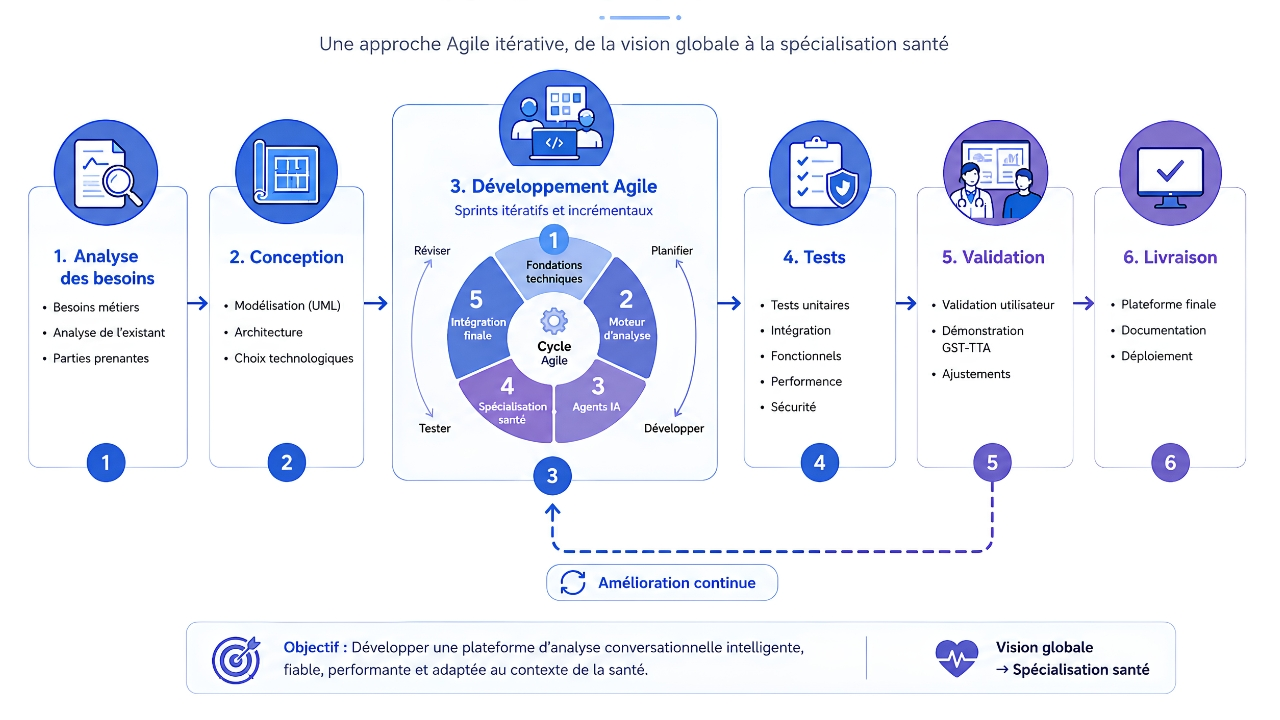
\includegraphics[width=0.82\textwidth]{images/methodologie.jpg}
\caption{Démarche générale adoptée pour la réalisation du projet}
\label{fig:methodologie}
\end{figure}

\subsection{Approche Agile adaptée}

Notre méthodologie s'inscrit dans une logique Agile, caractérisée par des cycles de développement courts (sprints) et une livraison incrémentale des fonctionnalités. Cette approche a été particulièrement adaptée à notre contexte, où les besoins ont évolué d'une vision générique vers une spécialisation progressive.

\begin{figure}[H]
\centering
\begin{tikzpicture}[
    node distance=0.8cm,
    phase/.style={rectangle, draw, thick, minimum width=5cm, minimum height=0.6cm, align=center, rounded corners, fill=LightGray!50},
    arrow/.style={->, thick, color=PrimaryRed, -{Stealth[length=3mm]}}
]
\node[phase, fill=PrimaryRed!15] (vision) {Vision globale de la plateforme};
\node[phase, below=of vision] (sprint1) {Sprint 1 : Fondations techniques};
\node[phase, below=of sprint1] (sprint2) {Sprint 2 : Moteur d'analyse};
\node[phase, below=of sprint2] (sprint3) {Sprint 3 : Agents IA};
\node[phase, below=of sprint3] (sprint4) {Sprint 4 : Spécialisation santé};
\node[phase, below=of sprint4, fill=PrimaryRed!25] (sprint5) {Sprint 5 : Intégration \& finalisation};

\draw[arrow] (vision) -- (sprint1);
\draw[arrow] (sprint1) -- (sprint2);
\draw[arrow] (sprint2) -- (sprint3);
\draw[arrow] (sprint3) -- (sprint4);
\draw[arrow] (sprint4) -- (sprint5);

% Feedback arrows
\draw[->, color=PrimaryRed, dashed, thick] (sprint2.west) -- ++(-1.2,0) |- (sprint1.west)
    node[pos=0.15, left, font=\scriptsize\itshape] {Retours};
\draw[->, color=PrimaryRed, dashed, thick] (sprint3.west) -- ++(-1.2,0) |- (sprint2.west);
\draw[->, color=PrimaryRed, dashed, thick] (sprint4.west) -- ++(-1.2,0) |- (sprint3.west);

% Annotation
\node[font=\small\itshape, color=MidGray, right=0.3cm of sprint3, xshift=2.5cm] {Spécialisation};
\node[font=\small\itshape, color=MidGray, right=0.3cm of sprint5, xshift=2.5cm] {Livraison};
\end{tikzpicture}
\caption{Structure des sprints : de la vision globale à la spécialisation santé}
\label{fig:sprints}
\end{figure}

\subsection{Organisation en sprints}

Le projet a été structuré en cinq sprints de deux à trois semaines, chacun ayant un objectif spécifique et livrant un incrément fonctionnel de la plateforme :

\begin{enumerate}
  \item \textbf{Sprint 1 : Fondations techniques} — Mise en place de l'infrastructure de base : structure du monorepo, environnement de développement, configuration des outils, et premier prototype d'interface.
  
  \item \textbf{Sprint 2 : Moteur d'analyse} — Développement du moteur computationnel (pandas, matplotlib) avec support multi-formats et fonctions statistiques essentielles.
  
  \item \textbf{Sprint 3 : Agents IA et orchestration} — Implémentation du framework agent (LangGraph), création des outils d'analyse, et mise en place de l'orchestrateur en trois phases.
  
  \item \textbf{Sprint 4 : Spécialisation santé} — Adaptation de la plateforme aux données du GST-TTA : intégration de jeux de données réels, personnalisation des analyses pour le contexte médical, et mise en place de la persistance.
  
  \item \textbf{Sprint 5 : Intégration et finalisation} — Assemblage complet des composants, tests d'intégration, optimisation des performances, et préparation de la livraison.
\end{enumerate}

Cette organisation a permis de maintenir un rythme de développement soutenu tout en assurant une validation continue des fonctionnalités produites.

\subsection{Phases de réalisation}

Au-delà de l'organisation en sprints, la réalisation du projet s'est articulée autour de quatre grandes phases complémentaires, permettant de structurer progressivement le développement de la plateforme.

\subsubsection{Phase 1 : Analyse des besoins}

Cette première phase a consisté à identifier les besoins des utilisateurs, à étudier le contexte du projet et à analyser les solutions existantes. Elle a permis de définir les objectifs du système ainsi que les principales exigences fonctionnelles et non fonctionnelles.

\subsubsection{Phase 2 : Conception et architecture}

La seconde phase a été consacrée à la modélisation de la solution et à la définition de son architecture logicielle. Les différents composants du système ont été conçus selon une approche modulaire afin de garantir leur maintenabilité, leur évolutivité et leur réutilisabilité.

\subsubsection{Phase 3 : Développement}

La troisième phase correspond à l'implémentation progressive de la plateforme selon une approche Agile. Les fonctionnalités ont été développées de manière incrémentale au cours de plusieurs sprints, permettant une validation continue des résultats obtenus et une adaptation aux besoins identifiés.

\subsubsection{Phase 4 : Tests et validation}

Enfin, une phase de validation a été menée afin de vérifier le bon fonctionnement de la plateforme. Différents niveaux de tests ont été réalisés pour évaluer la qualité de la solution, sa robustesse, ses performances ainsi que son adéquation aux objectifs fixés.

\begin{resultbox}{Synthèse méthodologique}
La méthodologie adoptée combine une approche Agile basée sur des développements itératifs avec une progression structurée en quatre phases : analyse, conception, développement et validation. Cette organisation a permis de faire évoluer progressivement la plateforme, depuis une vision générale jusqu'à une solution adaptée aux besoins du GST-TTA.
\end{resultbox}

%%%%%%%%%%%%%%%%%%%%%%%%%%%%%%%%%%%%%%%%%%%%%%%%%%%%%%%%%%%%%%%%%%%%%%%%%%%%%%
\section{Management du projet}
%%%%%%%%%%%%%%%%%%%%%%%%%%%%%%%%%%%%%%%%%%%%%%%%%%%%%%%%%%%%%%%%%%%%%%%%%%%%%%

La bonne conduite d'un projet de cette envergure nécessite une organisation rigoureuse, une répartition claire des responsabilités et un suivi temporel des différentes tâches. Cette section présente les principaux aspects du management du projet : l'équipe impliquée, la répartition des tâches et la planification temporelle.

\subsection{Équipe du projet}

Le projet a été mené par une équipe pluridisciplinaire, encadrée par des professionnels du GST-TTA et de l'établissement d'enseignement supérieur. L'équipe se compose comme suit :
\begin{table}[H]
\centering
\small
\renewcommand{\arraystretch}{1.25}

\begin{tabularx}{\textwidth}{
    >{\bfseries\raggedright\arraybackslash}p{3.3cm}
    >{\raggedright\arraybackslash}p{4.0cm}
    >{\raggedright\arraybackslash}X
}
\toprule
\rowcolor{TableHeader}
\color{white}\textbf{Rôle} &
\color{white}\textbf{Nom} &
\color{white}\textbf{Responsabilités} \\
\midrule

Stagiaires
&
El Gharib Mahmoud\par\medskip
Zarqi  Ezzoubair\par\medskip
El Attar Mohamed
&
\begin{itemize}[leftmargin=*,nosep]
    \item Analyse des structures et des sources de données ;
    \item Analyse et conception fonctionnelle et technique ;
    \item Modélisation et conception de l'architecture du système ;
    \item Développement de la plateforme et de ses différentes fonctionnalités ;
    \item Mise en place du moteur d'analyse et de l'orchestration agentique ;
    \item Intégration des modèles de langage et des composants d'intelligence artificielle ;
    \item Mise en place de la persistance, du cache et de la gestion des artefacts ;
    \item Réalisation des tests et validation des fonctionnalités ;
    \item Suivi des performances et amélioration de la solution ;
    \item Documentation et préparation de la soutenance.
\end{itemize}
\\

\midrule

Encadrante pédagogique
&
Pr.~Benabdoulah Ikram
&
Suivi académique du projet, orientation méthodologique,
correction et suivi du mémoire ainsi que préparation de la soutenance.
\\

\midrule

Encadrant technique
&
FANGACHI Oussama
&
Orientation technique, validation des fonctionnalités,
accompagnement du développement et exécution des tests.
\\

\bottomrule
\end{tabularx}

\caption{Composition de l'équipe projet et répartition des responsabilités}
\label{tab:equipe}
\end{table}
% \subsection{Répartition des tâches}

% La répartition des tâches a été organisée en fonction des compétences de chaque membre de l'équipe et des exigences du projet. Le tableau ci-dessous présente la répartition des principales activités :

% \begin{table}[H]
% \centering
% \caption{Répartition des tâches}
% \label{tab:repartition}
% \small
% \begin{tabularx}{\textwidth}{Y Z Z Z}
% \toprule
% \textbf{Tâche} & \textbf{Étudiant} & \textbf{Encadrant académique} & \textbf{Encadrant professionnel} \\
% \midrule
% Analyse des besoins & \textbullet & $\circ$ & \textbullet \\
% Conception architecturale & \textbullet & \textbullet & $\circ$ \\
% Développement backend & \textbullet & $\circ$ & $\circ$ \\
% Développement frontend & \textbullet & $\circ$ & $\circ$ \\
% Intégration des agents IA & \textbullet & $\circ$ & \textbullet \\
% Tests et validation & \textbullet & \textbullet & $\circ$ \\
% Rédaction du mémoire & \textbullet & \textbullet & $\circ$ \\
% \bottomrule
% \end{tabularx}
% \caption*{Légende : \textbullet\ Principal responsable, $\circ$ Contribution partielle}
% \end{table}

\subsection{Diagramme de Gantt}

La planification temporelle du projet a été établie sous forme de diagramme de Gantt, permettant de visualiser la séquence et la durée des différentes tâches. Ce diagramme couvre l'ensemble de la période de réalisation du projet, depuis l'analyse des besoins jusqu'à la livraison finale.

\begin{figure}[H]
\centering
\includegraphicsorplaceholder[width=0.95\textwidth]{gantt_projet_style_professionnel.png}
\caption{Diagramme de Gantt du projet}
\label{fig:gantt}
\end{figure}
La planification suit une organisation itérative dans laquelle plusieurs activités
peuvent être menées en parallèle. Cette organisation permet notamment
d'articuler progressivement la conception, le développement du moteur
d'analyse, l'intégration des agents d'intelligence artificielle,
l'implémentation du mécanisme de gestion du contexte, puis les phases
d'intégration, de validation et de documentation
\begin{resultbox}{Synthèse du management}
L'organisation du projet, structurée autour d'une équipe aux rôles clairement définis et d'une planification rigoureuse, a permis de mener à bien les différentes phases dans le respect des délais impartis. La répartition des tâches a favorisé une collaboration efficace entre les acteurs académiques et professionnels.
\end{resultbox}

%%%%%%%%%%%%%%%%%%%%%%%%%%%%%%%%%%%%%%%%%%%%%%%%%%%%%%%%%%%%%%%%%%%%%%%%%%%%%%
\section{Conclusion}
%%%%%%%%%%%%%%%%%%%%%%%%%%%%%%%%%%%%%%%%%%%%%%%%%%%%%%%%%%%%%%%%%%%%%%%%%%%%%%

Le Groupement Sanitaire Territorial Tanger--Tétouan--Al Hoceïma constitue un environnement particulièrement favorable au développement de projets innovants destinés à améliorer l'exploitation des données de santé. Grâce à sa stratégie de transformation numérique et à l'implication de la Direction de la Formation, de la Recherche et de l'Innovation, il offre un cadre propice à la conception de solutions d'aide à la décision intégrant les technologies de l'intelligence artificielle.

L'analyse du contexte et de l'existant a mis en évidence les limites des solutions actuelles, justifiant la nécessité de développer une plateforme adaptée aux besoins du secteur hospitalier. La problématique, les objectifs et la méthodologie adoptée constituent les fondements de la démarche entreprise.

L'organisation du projet, structurée autour d'une équipe pluridisciplinaire, d'une répartition claire des tâches et d'une planification temporelle rigoureuse, a permis d'assurer une conduite maîtrisée du projet dans le respect des échéances fixées.

Le chapitre suivant sera consacré à l'état de l'art des technologies et solutions existantes dans le domaine de l'analyse de données conversationnelle, des grands modèles de langage et des architectures d'agents intelligents qui constituent les fondements scientifiques de la plateforme développée.